\beginsong{Welle Wogte}[wuw={Rudyard Kipling, tuck (Ulrich Steckel)}, pfiii={67}, bo={372}]

\markboth{\songtitle}{\songtitle} 

\beginverse
\endverse

\centering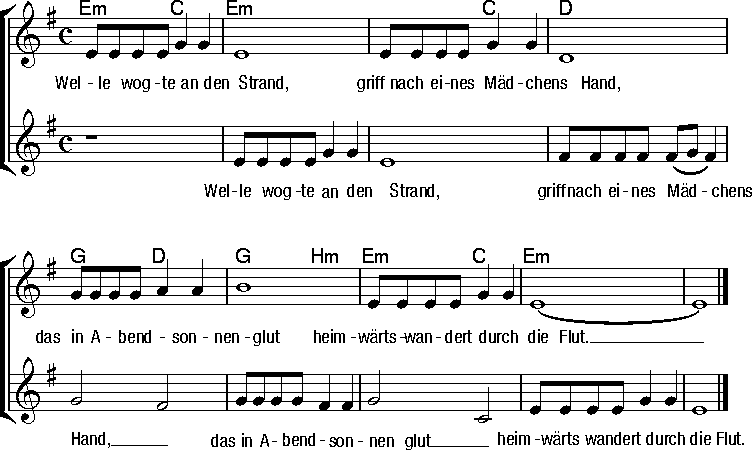
\includegraphics[width=1\textwidth]{Noten/Lied094.pdf}

\beginverse
\[Em]Zarte Brust und \[C]schlanker \[Em]Fuß, wahrt euch vor des \[C]Schmeichlers \[D]Gruß:
\[G]Höre Kind, mein \[D]sanft' Ge\[G]bot\[Hm]! \[Em]Warte! Bleib, ich \[C]bin der \[Em]Tod!
\endverse

\beginverse

^Drüben ruft der ^Liebe ^Glück. Schmachvoll wär's, blieb ^ich zu^rück.
^Dort im Fluss der ^helle ^Kla^ng. ^War's ein Fisch, der ^spielend ^sprang?
\endverse
\beginverse

^Schlanker Fuß und ^zartes ^Herz, harrt der Fähre ^heimat^wärts.
'^Hör auf mich', die ^Welle ^dro^ht, '^Warte Kind! Ich ^bin der ^Tod.'
\endverse
\beginverse

^Liebster ruft, da ^muss ich ^eilen. Schande träf mich, ^wollt ich ^weilen.
^Welle, Welle ^wogt und ^ri^ngt, ^mächtig ihren ^Leib um^schlingt.
\endverse
\beginverse

^Töricht Herze, ^treue ^Hand, kleiner Fuß trat ^nie ans ^Land.
^Welle wandert, ^Welle ^ro^t, ^wogt hinab und ^trägt den ^Tod.
\endverse

\endsong
\beginscripture{}
Der Verfasser des Liedes Rudyard Kipling erhielt 1907 als bis dahin jüngster Autor den Literaturnobelpreis. Von ihm stammt auch das berühmte Kinderbuch "Das Dschungelbuch".
\endscripture
\begin{intersong}

\ifthenelse{\boolean{pics}}{
\ThisLRCornerWallPaper{1}{Bilder/welle_cut.png}
}{}

\end{intersong}